\documentclass{article}
\usepackage{graphicx}
\usepackage{tikz}
\usetikzlibrary{arrows,automata}


\begin{document}

\title{\huge{Boat Lift} \\ {\fontsize{13}{1} \selectfont Global requirements for the whole system} }
\author{Filippo Bernardi, Jasper Lustig, Jonas Wallmeier, Snorri Stefansson}

\maketitle

%\begin{abstract}

%\end{abstract}

\vspace{3cm}

\begin{figure}[!h]
\centering

	%\path[->, dashed]  (S)  edge              node {a} (l1);
	%\path[->, dotted]  (l1) edge [bend left]  node {a} (S);
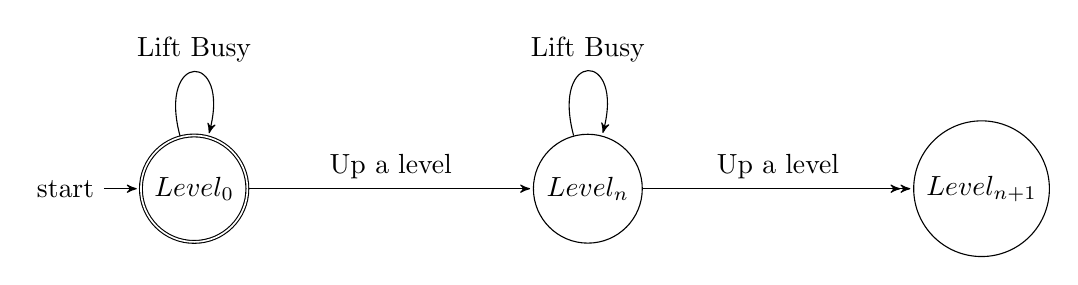
\begin{tikzpicture}[>=stealth',shorten >=1pt,auto,node distance=5cm]
	\node[initial,state,accepting] (S)      {$Level_0$};
	\node[state]         (l1) [right of=S]  {$Level_n$};
	\node[state]         (l2) [right of=l1] {$Level_{n+1}$};
		
	\path      (S)  edge [loop above] node {Lift Busy} (S);
	\path[->]  (S)	edge              node {Up a level} (l1);
	\path      (l1)	edge [loop above] node {Lift Busy} (l1);
	\path[->>] (l1) edge              node {Up a level} (l2);

	edge [bend left]  node {b} (l1);
\end{tikzpicture}
\caption{An extreme simple automata for the boat lift referenced in this document}
\end{figure}

\pagebreak

\section{}

\textbf{Definition:}
Ship lift. General purpose ship lift for elevating ships to a geographically, vertical, higher location. \\

\textbf{Global requirements for the system:}
\begin{enumerate}
	\item Only one boat can be elevated at a time
	\item The lift has to be big enough for all boats going through.
	\item The water level in the lift can only change when both gates are closed securely.
	\item Gates should not close while a boat is going through them.
	\item The boats are signaled when to enter or leave the lift.
	\item Only one gate can be open at a time.
	\item There has to be some valve able to level at the same height two connected basins.
	\item Every floor should be able to decrease its water level.
	\item The water flow can not distort the boats equilibrium.
	\item Sensing if the ship is completely inside the lift or not.
	\item The gates should not be able to open when the water level on the floor above or below is not the same.
	
\end{enumerate}

\pagebreak

\textbf{Sequence for the boat lift}, elevating a boat up a floor.

\begin{enumerate}
	\item Doors will open of no boat is in the lift
	\item A boat enters the first level 0 lift.
	\item The doors in level 0 closed.
	
	\item Level 0 fills up with water from level 1. The boat is elevated to level 1.
	\item Door into level 1 open when the water level is the same in both level 0 and 1.
	\item The boat sails into level 1.
	\item The doors in level 1 close.
	
	\item Level 1 fills up with water from level 2. The boat is elevated to level 1.
	\item Door into level 2 open when the water level is the same in both level 1 and 2.
	\item The boat sails into level 2.
	\item The doors in level 2 close.
	
	\item The door out of level 2 open. The boat sails on its way. 
\end{enumerate}

Items from 4-7 and 8-11 are repetitive for indication of this being enough for proofing of a N-order system. Were this could be determined as a second order system.

\pagebreak

Questionable components of the project?
\begin{itemize}
	\item Should the be a Operator? For trying to eliminate some security flaws.
	\item Multiple floor. Sufficient would be lifting up two times to cover all aspects? Rather N-times?  What is relevant or doable?
\end{itemize}


\end{document}\grid
\grid
